\subsection{Примеры неустойчивых решений уравнения теплопроводности}
\vspace{1em}

\newtheorem{exmp}{Пример}

\begin{exmp}
\end{exmp}

В качестве начального условия возмем $u(x, 0) = \sin{(\pi x)}$. Вспомним, что при $\alpha < \pi^2$ система устойчива. На рисинке 1 численный пример задачи \eqref{sys} - \eqref{s_control} без управления ($m = 0$, $r = 0$), на рисунке 2 - с управлением ($m = 2$, $r = 1$), где $\alpha = \pi^2 - 2$.


\begin{figure}[H]
\centering
\begin{minipage}{.5\textwidth}
  \centering
  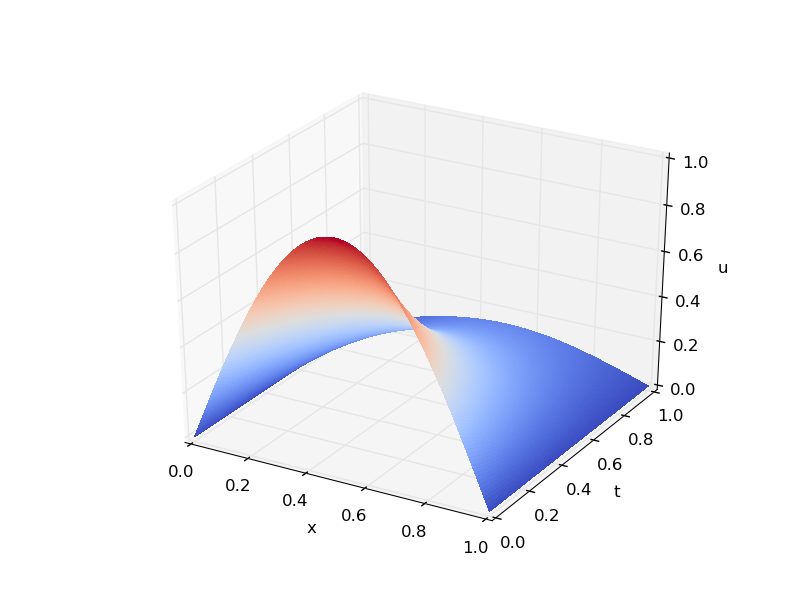
\includegraphics[width=3.5in]{par_ex_pim2}
  \caption{Без управления}
  \label{fig:test1}
\end{minipage}%
\begin{minipage}{.5\textwidth}
  \centering
  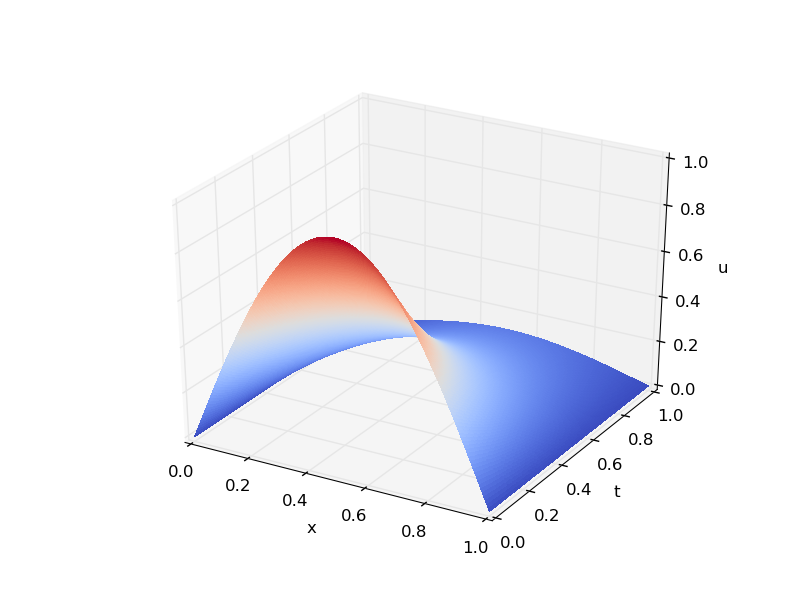
\includegraphics[width=3.5in]{par_re_pim2}
  \caption{Управление $m = 2,\; r = 1$}
  \label{fig:test2}
\end{minipage}
\end{figure}

\begin{exmp}
\end{exmp}

Начальные условия те же, что и в предыдущем примере. Продемонстрируем неустойчивость нулевого решения (рис.3) и стабилизацию (рис.4) при $\alpha = \pi^2 + 0.1$. Фиксируем $\omega = [0, 0.2]$. Необходимо подобрать параметры $m$, $r_m$ так, чтобы $\beta > 0$ и $q > 0$. Рассмотрим подробнее $q = [(\pi(m + 1))^2 - \alpha - 1]$. При заданном $\alpha = \pi^2 + 0.1$, достаточно взять $m = 2$ для выполнения неравенства. Параметр $r$ придется подобрать так, чтобы решение стремилось к нулю.


\begin{figure}[H]
\centering
\begin{minipage}{.5\textwidth}
  \centering
  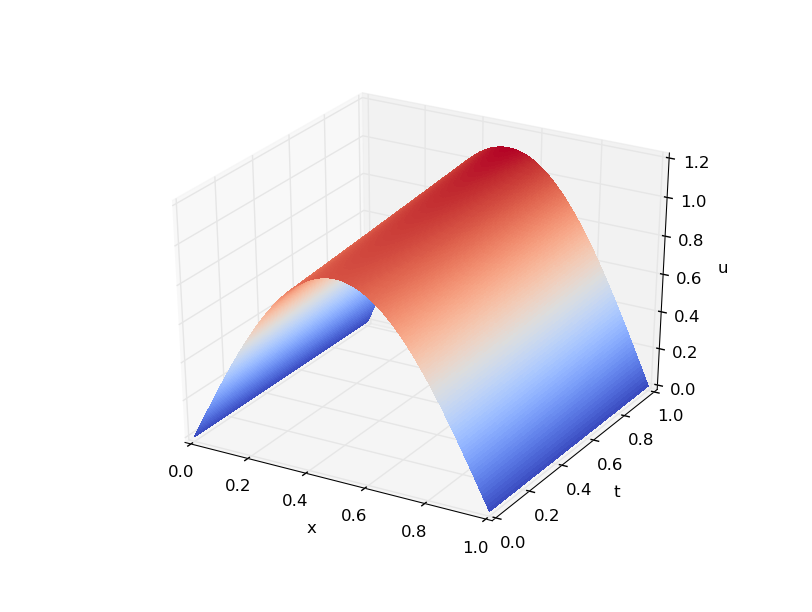
\includegraphics[width=3.5in]{par_ex_pi01}
  \caption{Без управления}
  \label{fig:test1}
\end{minipage}%
\begin{minipage}{.5\textwidth}
  \centering
  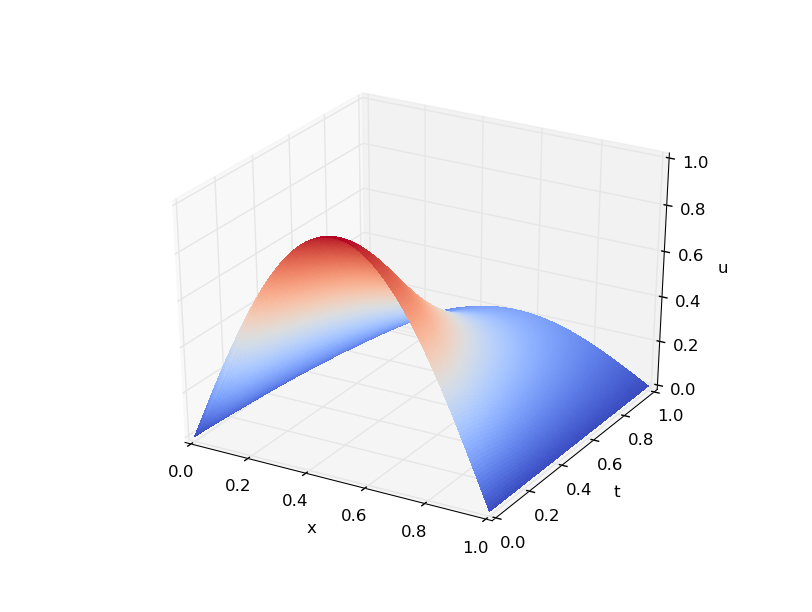
\includegraphics[width=3.5in]{par_re_pi01}
  \caption{Управление $m = 2,\; r = 8$}
  \label{fig:test2}
\end{minipage}
\end{figure}

\begin{exmp}
\end{exmp}

Пусть $u(x, 0) = x(1 - x)$ - начальное условие . Заведомо выберем параметр $\alpha = \pi^2 + 3$ большим. Зафиксируем $\omega = (0, 0.4)$. Необходимо подобрать $m$, таким чтобы $q > 0$. При $m \ge 2$ условие выполняется, поэтому мы фиксируем $m = 2$. На рис.5 показано, как быстро растет решение задачи \eqref{sys} - \eqref{s_control} при небольшом увеличении $\alpha$. Стабилизация этой системы представлена на рисунке 6.  

\begin{figure}[H]
\centering
\begin{minipage}{.5\textwidth}
  \centering
  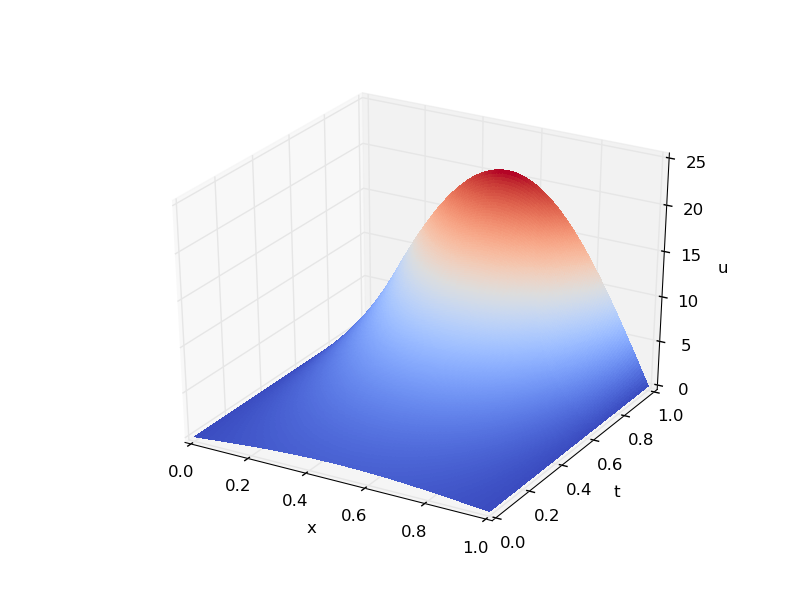
\includegraphics[width=3.5in]{par_ex_pi3}
  \caption{Без управления}
  \label{fig:test1}
\end{minipage}%
\begin{minipage}{.5\textwidth}
  \centering
  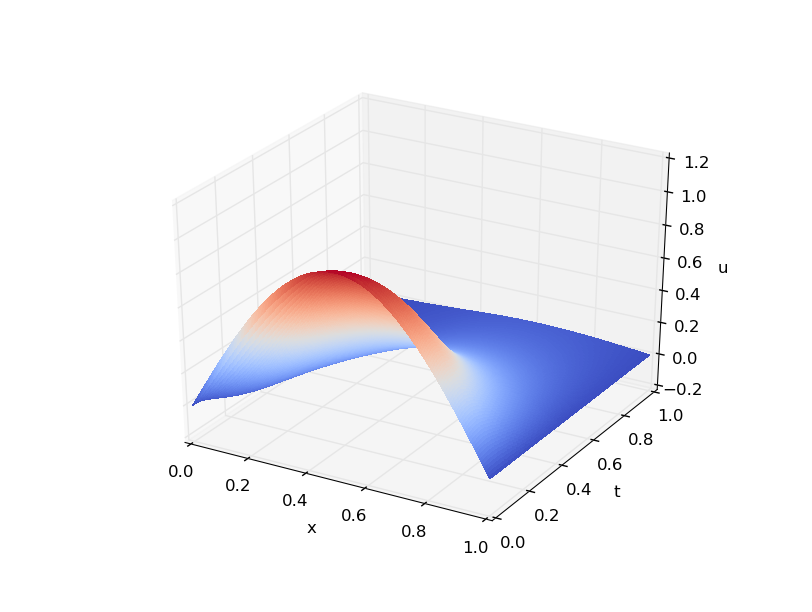
\includegraphics[width=3.5in]{par_re_pi3}
  \caption{Управление $m = 2,\; r = 15$}
  \label{fig:test2}
\end{minipage}
\end{figure}